\section{Results}
Lorem ipsum dolor sit amet, consetetur sadipscing elitr, sed diam nonumy eirmod tempor invidunt ut labore et dolore magna aliquyam erat, sed diam voluptua. At vero eos et accusam et justo duo dolores et ea rebum. Stet clita kasd gubergren, no sea takimata sanctus est Lorem ipsum dolor sit amet. Lorem ipsum dolor sit amet, consetetur sadipscing elitr, sed diam nonumy eirmod tempor invidunt ut labore et dolore magna aliquyam erat, sed diam voluptua. At vero eos et accusam et justo duo dolores et ea rebum. Stet clita kasd gubergren, no sea takimata sanctus est Lorem ipsum dolor sit amet.

\subsection{Citation examples}
And here we demonstrate like (\cite{hoehle_espoused_2015}) how citations look alike in this \LaTeX file. You can also list all authors (\cite{venkatesh_usability_2014}). And click any of the references and see what happens in your PDF reader, like here: \cite{university_of_arkansas_mobile_2015}.

\subsection{An example table}
Lorem ipsum dolor sit amet, consetetur sadipscing elitr, sed diam nonumy eirmod tempor invidunt ut labore et dolore magna aliquyam erat, sed diam voluptua. 

\begin{table}[h!]
\centering
\begin{tabular}{|c|c|c|c|} 
 \hline
ID & 1st run & 2nd run & 3rd run \\ [0.5ex] 
 \hline
 1 & 6 & 87837 & 787 \\ 
 \hline
 2 & 7 & 78 & 5415 \\
 \hline
 3 & 545 & 778 & 7507 \\
 \hline
 4 & 545 & 18744 & 7560 \\
 \hline
 5 & 88 & 788 & 6344 \\ 
 \hline
\end{tabular}
\caption{Our amazing results in one, lean table}
\label{table:1}
\end{table}

\section{Conceptional Background}


\subsection{A sub-section}
\begin{figure}[h]
    \centering
    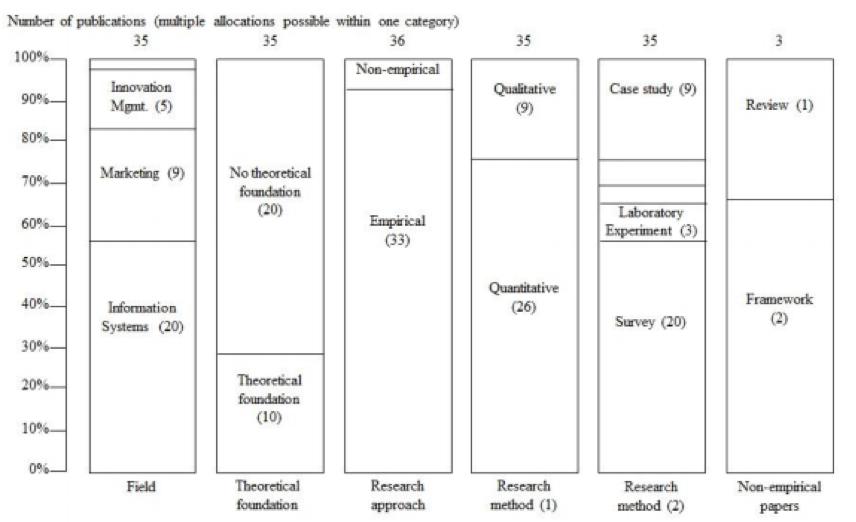
\includegraphics[width=0.8\textwidth]{Picture1.png}
    \caption{Publication diagram}
    \label{fig:mesh1}
\end{figure}

\subsection{Yet another sub-section}
As you can see in the figure \ref{fig:mesh1}, everything looks better in a diagram. Also, in the page \pageref{fig:mesh1} 
is the same example.


\sectionunnumbered{Appendix}
\begin{table}[h!]
\centering
\begin{tabular}{|c|c|c|c|} 
 \hline
Source & 1st run & 2nd run & 3rd run \\ [0.5ex] 
 \hline
 Kentucky & 6 & 87837 & 787 \\ 
 \hline
 California & 7 & 78 & 5415 \\
 \hline
 New Jersey & 545 & 778 & 7507 \\
 \hline
 Manitoba & 545 & 18744 & 7560 \\
 \hline
 Alaska & 88 & 788 & 6344 \\ 
 \hline
\end{tabular}
\caption{Raw data (remark: this one is in the Appendix -> Roman page nr)}
\label{table:raw_data}
\end{table}